\subsubsection{既知の座標を用いたドリフトの除去}


% TODO: 軌跡推定と位置推定の使いわけ
図\ref{fig:pdr-move}に示すように,PDRによる軌跡推定では角速度センサーの誤差に起因するドリフト現象が発生する.
この現象は,角速度から進行方向を求める際のわずかな誤差が時間経過とともに累積し,
推定軌跡が本来の軌跡から徐々に逸脱する.この問題への対処として,
本ライブラリではドリフト補正機能を実装しており,DriftCorrectorクラスとして提供している.


% TODO:表現が冗長
DriftCorrectorクラスの利用例をListing \ref{lst:drift-corrector}に示す.
このクラスに必要な情報は既知の座標データである.既知の座標データには
特定の時刻における歩行者の位置情報が含まれている.このデータは
任意の時刻の座標である必要はなく,軌跡の始点や終点など,いくつかの
時点での位置情報があれば補正が可能である.また,補正の精度は
与えられる既知の座標の数や,座標間の時間間隔によって変化する.


% TODO 2.captionの名前は検討した方がいいかも
% TODO 2.やっぱり関数ものせた方がいいかも,何の情報を入力するという部分は必要かもしれない(要検討)
% TODO: 2.しかし軌跡を引数に与えていないから違和感がある.内部的にはenhanceSensorDataの角度をみて修正してる.コードごと消すか
\begin{lstlisting}[caption={DriftCorrectorの使用例},label=lst:drift-corrector,float=h]
# 正解座標データ
ground_truth = pd.DataFrame({
    'ts': [0, 180],           # タイムスタンプ(秒)
    'x': [15.0, 15.0],       # x座標(メートル)
    'y': [19.0, 19.0]        # y座標(メートル)
})

# DriftCorrectorの初期化と補正の実行
drift_corrector = DriftCorrector(
    pdr_estimator=estimator,  # PDREstimatorインスタンス
    gt_data=ground_truth      # 既知座標データ
)
\end{lstlisting}

% TODO: ちょっと意味がわからない文章
DriftCorrectorクラスは,既知座標との比較に基づいて角速度データの累積誤差を
補正する.この補正処理は式\eqref{eq:drift_correction}で表される.
$\theta'(t)$は時間$t$における補正後の角度,$\theta(t)$は
補正前の角度,$d$はドリフトの大きさを表す.この式は時間経過に伴う
ドリフトの累積効果を線形モデルで近似し,補正を行う.
最適なドリフト値$d$の決定には,既知の座標との誤差を最小化するアプローチを
採用している.具体的には,補正後の軌跡の終点と既知の座標との
ユークリッド距離$E$を式\eqref{eq:euclidean_distance}で計算する.
$(x_n, y_n)$は既知の座標,$(x_{n+1}, y_{n+1})$は補正された
軌跡の終点を表す.DriftCorrectorはこの距離$E$が最小となるドリフト値をグリッドサーチにより探索する.
探索範囲はデフォルトで[-0.02, 0.02] rad/sとしている.この範囲は一般的なMEMSジャイロセンサーの
バイアス誤差の特性を考慮して設定されている.より大きな範囲を設定すると,
センサーの誤差だけでなく,実際の方向転換まで補正してしまう可能性がある.
また,この値の範囲は外部から変更可能であり,使用するセンサーの特性に応じて調整できる.
図\ref{fig:pdr-remove-drift}に示すように,ドリフト補正後の軌跡は
元の軌跡と比較して正解軌跡の形状に近づいている.この補正は既知の座標間の
距離が近い場合に効果的である.また,2点以上の既知の座標が存在する場合も,
同様のアプローチで補正が可能である.

\begin{equation}
    \theta'(t) = \theta(t) - (d \times t)
    \label{eq:drift_correction}
\end{equation}


\begin{equation}
    E = \sqrt{(x_{n+1} - x_n)^2 + (y_{n+1} - y_n)^2}
    \label{eq:euclidean_distance}
\end{equation}

% TODO:2.ここにパワポにあるようなグリードサーチしている感がある図を載せるといいかも

\begin{figure}[H]
	\centering
	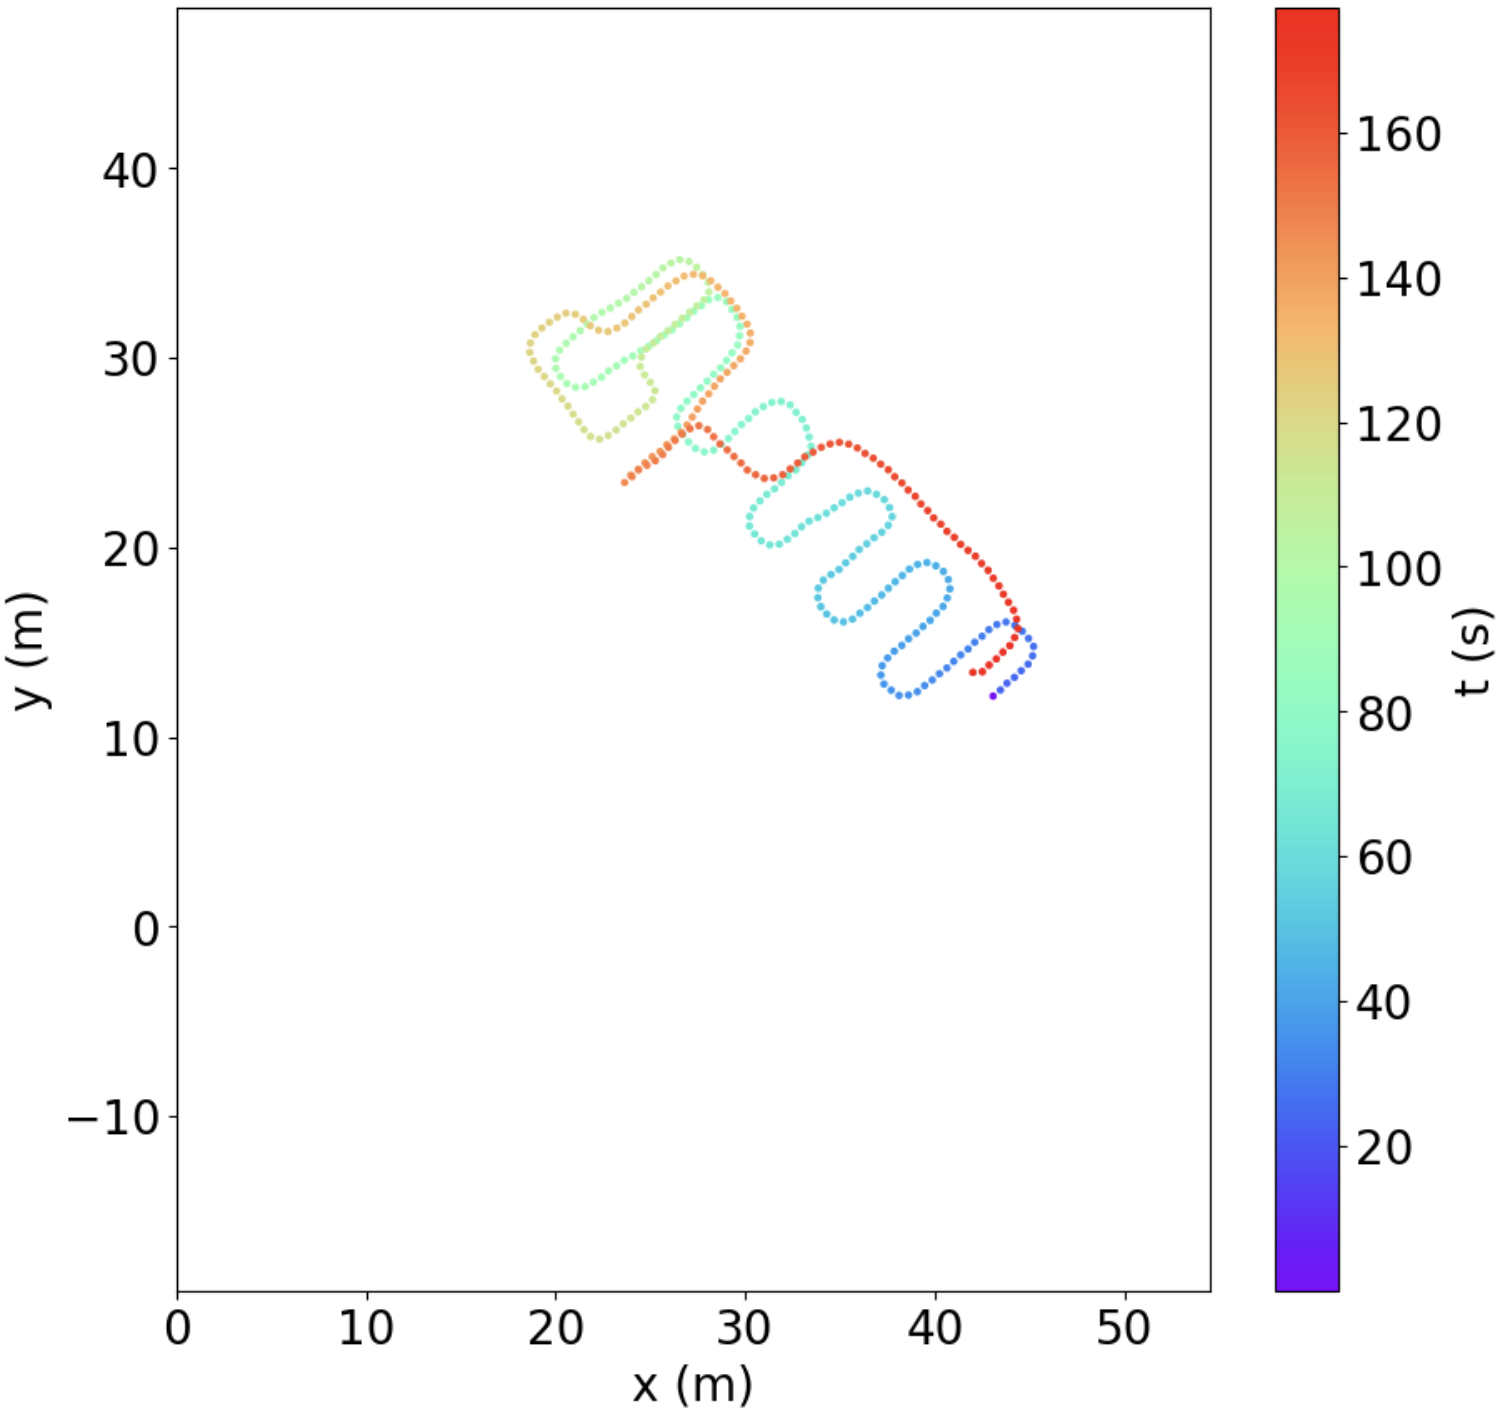
\includegraphics[width=\linewidth]{../image/pdr-remove-drift-two.jpg}
	\caption{ドリフト補正後の軌跡}    \label{fig:pdr-remove-drift}
\end{figure}

